\documentclass{article}

\topmargin -.5in
\textheight 8.25in
\oddsidemargin 0in
\evensidemargin 0in
\textwidth 6.5in
\parindent 3em

\usepackage{amsmath}

%% Please use the following statements for
%% managing the text and math fonts for your papers:
\usepackage{times}
%\usepackage[cmbold]{mathtime}
\usepackage{bm}
\usepackage{natbib}

%\usepackage{algorithm}
%\usepackage{fancyhdr}
\usepackage{graphics,color,pict2e}
\usepackage{epsfig}
%\usepackage{times}
%\usepackage[cmbold]{mathtime}
%\usepackage{bm}
%\usepackage{rotating}
%\usepackage{pdflscape}
%\usepackage{longtable}
\usepackage{booktabs}
\usepackage{lscape}
\usepackage{pdflscape}    
%\usepackage{C:/R/R-2.11.1/share/texmf/Sweave}

%\theoremstyle{plain}
%\newtheorem{Theorem}{Theorem}[section]
\newtheorem{theorem}{Theorem}
\newtheorem{corrolary}{Corrolary}
\newtheorem{result}{result}
\newtheorem{Lemma}{Lemma}
\newcommand{\toi}{t}
\newcommand{\eqd}{\buildrel D \over =}
\newcommand{\vect}{\bf }
\newcommand{\sle}{\stackrel{st}{\le}}




\newcommand{\ch}[2]{\ensuremath{ \left( \begin{array}{c} #1 \\ #2 \end{array} \right) }}
\newcommand{\dfn}[2]{\ensuremath{ \left( #1 \right)_{(#2)}}}



\begin{document}

{\bf \large Notes on: Prevalence Estimates from Surveys with Imperfect Assays}

\today


%\begin{abstract}
%asdf
%\end{abstract}

Damon,

Here are some notes on the project. You can change the notation if you want. I am just putting down something so we can be clear about what we are doing.

\section{Overview}

Quick overview. I described the problem in Section~\ref{sec-math}. The usual adjustment for sensitivity and specificity is described in Section~\ref{sec-usualAdj}. Then the three parts I spoke about. First, the confidence interval for a simple random sample is described in Section~\ref{sec-thetastar} (that is what you already did). Second, the confidence interval assuming a perfect assay in Section~\ref{sec-betaPerfect}. And finally, the
confidence interval for an imperfect assay in Section~\ref{sec-betaImperfect}.


\section{Mathematical Statement of Problem}
\label{sec-math}

Suppose we take a survey, that is divided into $k$ sampling units (e.g., states in the US).
We take a simple random sample of individuals from each unit, perform and assay on each individual to determine who has a disease, and measure the number of individuals who have a positive value for the assay.

Let $X_i$ be the number of positives by the assay, out of $n_i$ measured in sampling unit $i$.
Suppose we had a perfect assay with 100\% sensitivity and 100\% specificity. Then let $X_i^*$ be the true number with the disease out of the $n_i$ sampled in unit $i$.

Let $X_i^* \sim Binomial(n_i, \theta_i^*)$ for $i=1,\ldots,k$. We are interested in the prevalence of disease in the population. Suppose there are $N_i$ individuals in the population of unit $i$. Then the prevalence of the population is
\begin{eqnarray*}
\beta & = & \frac{ \sum_{i=1}^{k} N_i \theta_i^* }{ \sum_{j=1}^{k} N_j }  =  \sum_{i=1}^{k} w_i \theta_i,
\end{eqnarray*}
where $w_i = N_i/N$ and $N=\sum_{j=1}^{k} N_j$.


Suppose we evaluate the assay. We measure the assay on $m_n$ individuals known not to have the disease (negative controls), and on $m_p$ individuals known to have the disease (positive controls). Let $C_n$ and $C_p$ be the number who tested positive out of the $m_n$ in the negative control and the $m_p$  in the positive control. Now make a convenience assumption:
\begin{itemize}
\item Assume that the negative and positive controls act like simple random samples from their populations (e.g., the $m_n$ negative controls are like a simple random sample from the total population of individuals without the disease).
\end{itemize}
Under that assumption, $C_n \sim Binomial(m_n, \phi_n)$ and $C_p \sim Binomial(m_p, \phi_p)$,
where $1-\phi_n$ is the specificity (true negative rate of the assay),
and $\phi_p$ (true positive rate of the assay) is the sensitivity.

Here is the statistical problem. Assuming all of the above holds, and we observe realizations of $X_1,\ldots, X_k$ and $C_n$ and $C_p$, and the other values are known constants ($n_1,\ldots, n_k$, $w_1,\ldots, w_k$,  $m_n$, and $m_p$), what is a good estimate and confidence interval procedure for $\beta$.


\section{Usual Adjustment for Sensitivity and Specificity}
\label{sec-usualAdj}

To simplify the problem, suppose there is only one sampling unit, and let $X_1=X$ and $n_1=n$, etc. Then $\beta = \theta_1^*=\theta^*$.
Further assume that $\phi_p$ and $\phi_n$ are known. Let $Y_1,\ldots,Y_n$ be the result of the assay from the $n$ individuals in the population
($Y_i=1$ is positive and $Y_i=0$ is negative). Let $Y_1^*,\ldots,Y_n^*$ be the true disease status ($Y_i^*=1$ is diseased, and $Y_i^*=0$ is not diseased).
Then using the definition of sensitivity and specificity, we get:
\begin{eqnarray*}
Pr[ Y_i =1 | Y_i^*=1] & = & \phi_p \\
Pr[ Y_i=0 | Y_i^*=0] & = & 1- \phi_n
\end{eqnarray*}
and
\begin{eqnarray*}
Pr[ Y_i=1] & = & Pr[ Y_i =1 | Y_i^*=1]  Pr[Y_i^*=1] + Pr[ Y_i =1 | Y_i^*=0] Pr[ Y_i^*=0] \\
& = & \phi_p \theta^* + \phi_n (1-\theta^*)  \\
& = & \theta^* (\phi_p - \phi_n) + \phi_n.
\end{eqnarray*}
Let $\theta = Pr[ Y_i=1]$.

So we have
\begin{eqnarray*}
& & X \sim Binomial \left(n, \theta \right)  \\
\mbox{ where} & \theta & = \theta^* \left\{ \phi_p - \phi_n \right\} + \phi_n.
\end{eqnarray*}
Thus,
\begin{eqnarray}
\theta^* & =  & \frac{ \theta - \phi_n }{ \phi_p - \phi_n}  = \frac{ \theta + (1 - \phi_n) -1  }{ \phi_p + (1 - \phi_n) -1 } \label{eq:thetastar}
\end{eqnarray}

Suppose we estimate the sensitivity as $\widehat{Se} = \hat{\phi}_p = C_p/m_p$ and the specificity as $\widehat{Sp} = 1-\hat{\phi}_n = 1- C_n/m_n$,
and we define the apparent prevalence as the sample proportion of the positive assay results, $\hat{\theta} = x/n$.
This gives the usual estimator for  prevalence adjusted for sensitivity and specificity
 \citep[see e.g.,][]{Roga:1978},
\begin{eqnarray*}
\hat{\theta}^* & = & \frac{ \hat{\theta} - \hat{\phi}_n }{\hat{\phi}_p - \hat{\phi}_n} = \frac{ \hat{\theta} + \widehat{Sp} -1 }{\widehat{Se} + \widehat{Sp} -1}.
\end{eqnarray*}


\section{Confidence Interval on $\theta^*$}
\label{sec-thetastar}

The simulation you (Damon) already did handles this problem. It answers: what is a good confidence interval for $\theta^*$?
You compared the method of \citet{Lang:2014} to the new method described in the Supplement to \citet{Kali:2021}, using the method of \citet{FayP:2015}.
It shows that the lower error has a better bound with the new method.

\section{Confidence Interval on $\beta$ with a Perfect Assay}
\label{sec-betaPerfect}


Suppose we have a perfect assay (i.e., $\phi_p=1$ and $\phi_n=0$). Then $\theta^* = \theta$, and $\beta = \sum_{i=1}^{k} w_i \theta$.
The problem reduces to getting a confidence interval for a weighted average of the means of sample proportions.
This problem is a standard survey sampling one. Some methods are \citet{Korn:1998}, see the review in \citet{Dean:2015}.

Another way to address this problem is to assume that $X_i \sim Poisson( n_i \theta_i)$ and use the methods
of \citet{FayF:1997} or \citet{FayK:2017}.
The notation is different in those papers. Here is the correspondence between the notations in these notes and in \citet{FayK:2017}.

\begin{tabular}{cc}
These Notes & Fay and Kim  \\ \hline
$w_i$     & $s_i$ \\
$\theta_i$ & $\lambda_i$ \
\end{tabular}

and $X_i$ and $n_i$ are the same in both papers. 


This should give a confidence interval for $\beta=\sum_{i=1}^{k} w_i \theta_i$
that gives a lower and upper confidence distribution that is distributed gamma. (I will let you work out those details. Let me know if it is not easy.)

\subsection{Dirichlet Weights Simulation Results}

I present results for two scenarios:

\begin{itemize}
    \item The weight of each group is generated from a Dirichlet distribution with equal concentration parameters for all dimensions. The "Coefficient of Variation" in the figures referes to these weights.
    \item The true positivity of each group is generated from a Beta distribution which achieves the specified mean and ICC.
    \item Figure~\ref{fig:dws1}. Samples of 8,000 groups of 1. Population prevalence = 0.05\%/ Varying weight variance. Replicated 10,000 times.
    \begin{itemize}
        \item The two wsPoisson methods maintain appropriate or conservative coverage, regardless of the coefficient of variation among the weights.
        \item The other two methods (Agresti-Coull and Clopper-Pearson) only begin to falter at unrealistic or unusual (according to Barry) coefficients of variation.
        \item More typical coefficients of variation would be 20\%-40\%.
    \end{itemize}
    \item Figure~\ref{fig:dws2}. Samples of 200 groups of 50. Population prevalence = 0.05\%. Varying ICC. Varying weight variance. Replicated 10,000 times.
    \begin{itemize}
        \item Results here are a bit confusing.
        \item I know that the results for Agresti-Coull and Clopper-Pearson could be improved with a better estimate for \(\hat{\text{var}}(\hat{p}) \). The simple estimate I was using appears to perform poorly in the case of high ICC. \textbf{I wonder if Barry can point me towards a good estimator for \(\hat{\text{var}}(\hat{p}) \) in the presence of high ICC.}
        \item It is a bit strange that the wsPoisson methods perform better when there is extreme Coefficient of Variation, but it is consistent with the previously observed behavior of higher CoV leading to more conservative coverage.
    \end{itemize}
\end{itemize}

\begin{figure}
    \centering
    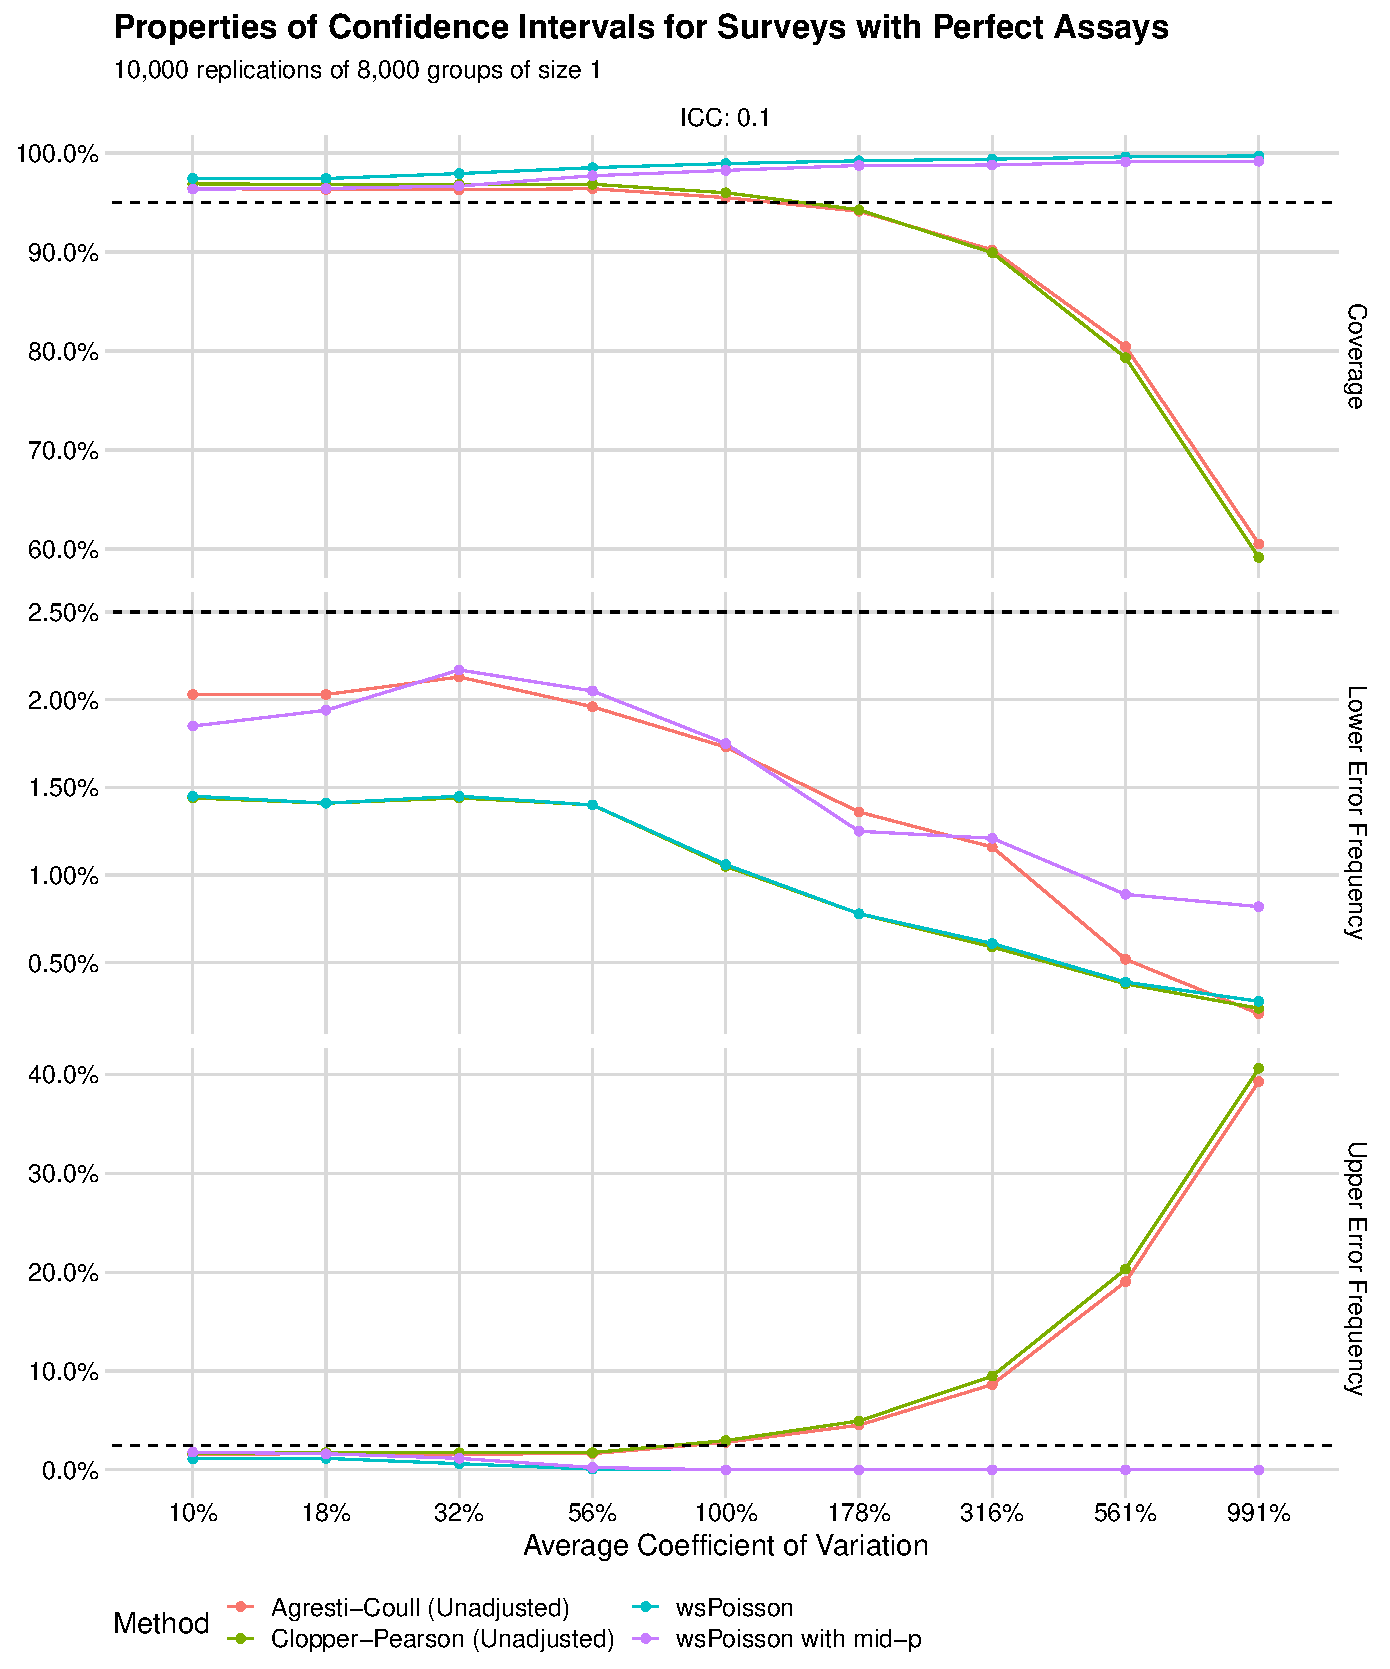
\includegraphics[width=\textwidth]{figures/results_plot_8000_1.pdf}
    \caption{Dirichlet Weights Scenario 1}
    \label{fig:dws1}
\end{figure}

\pagebreak
\begin{landscape}
\begin{figure}
    \centering
    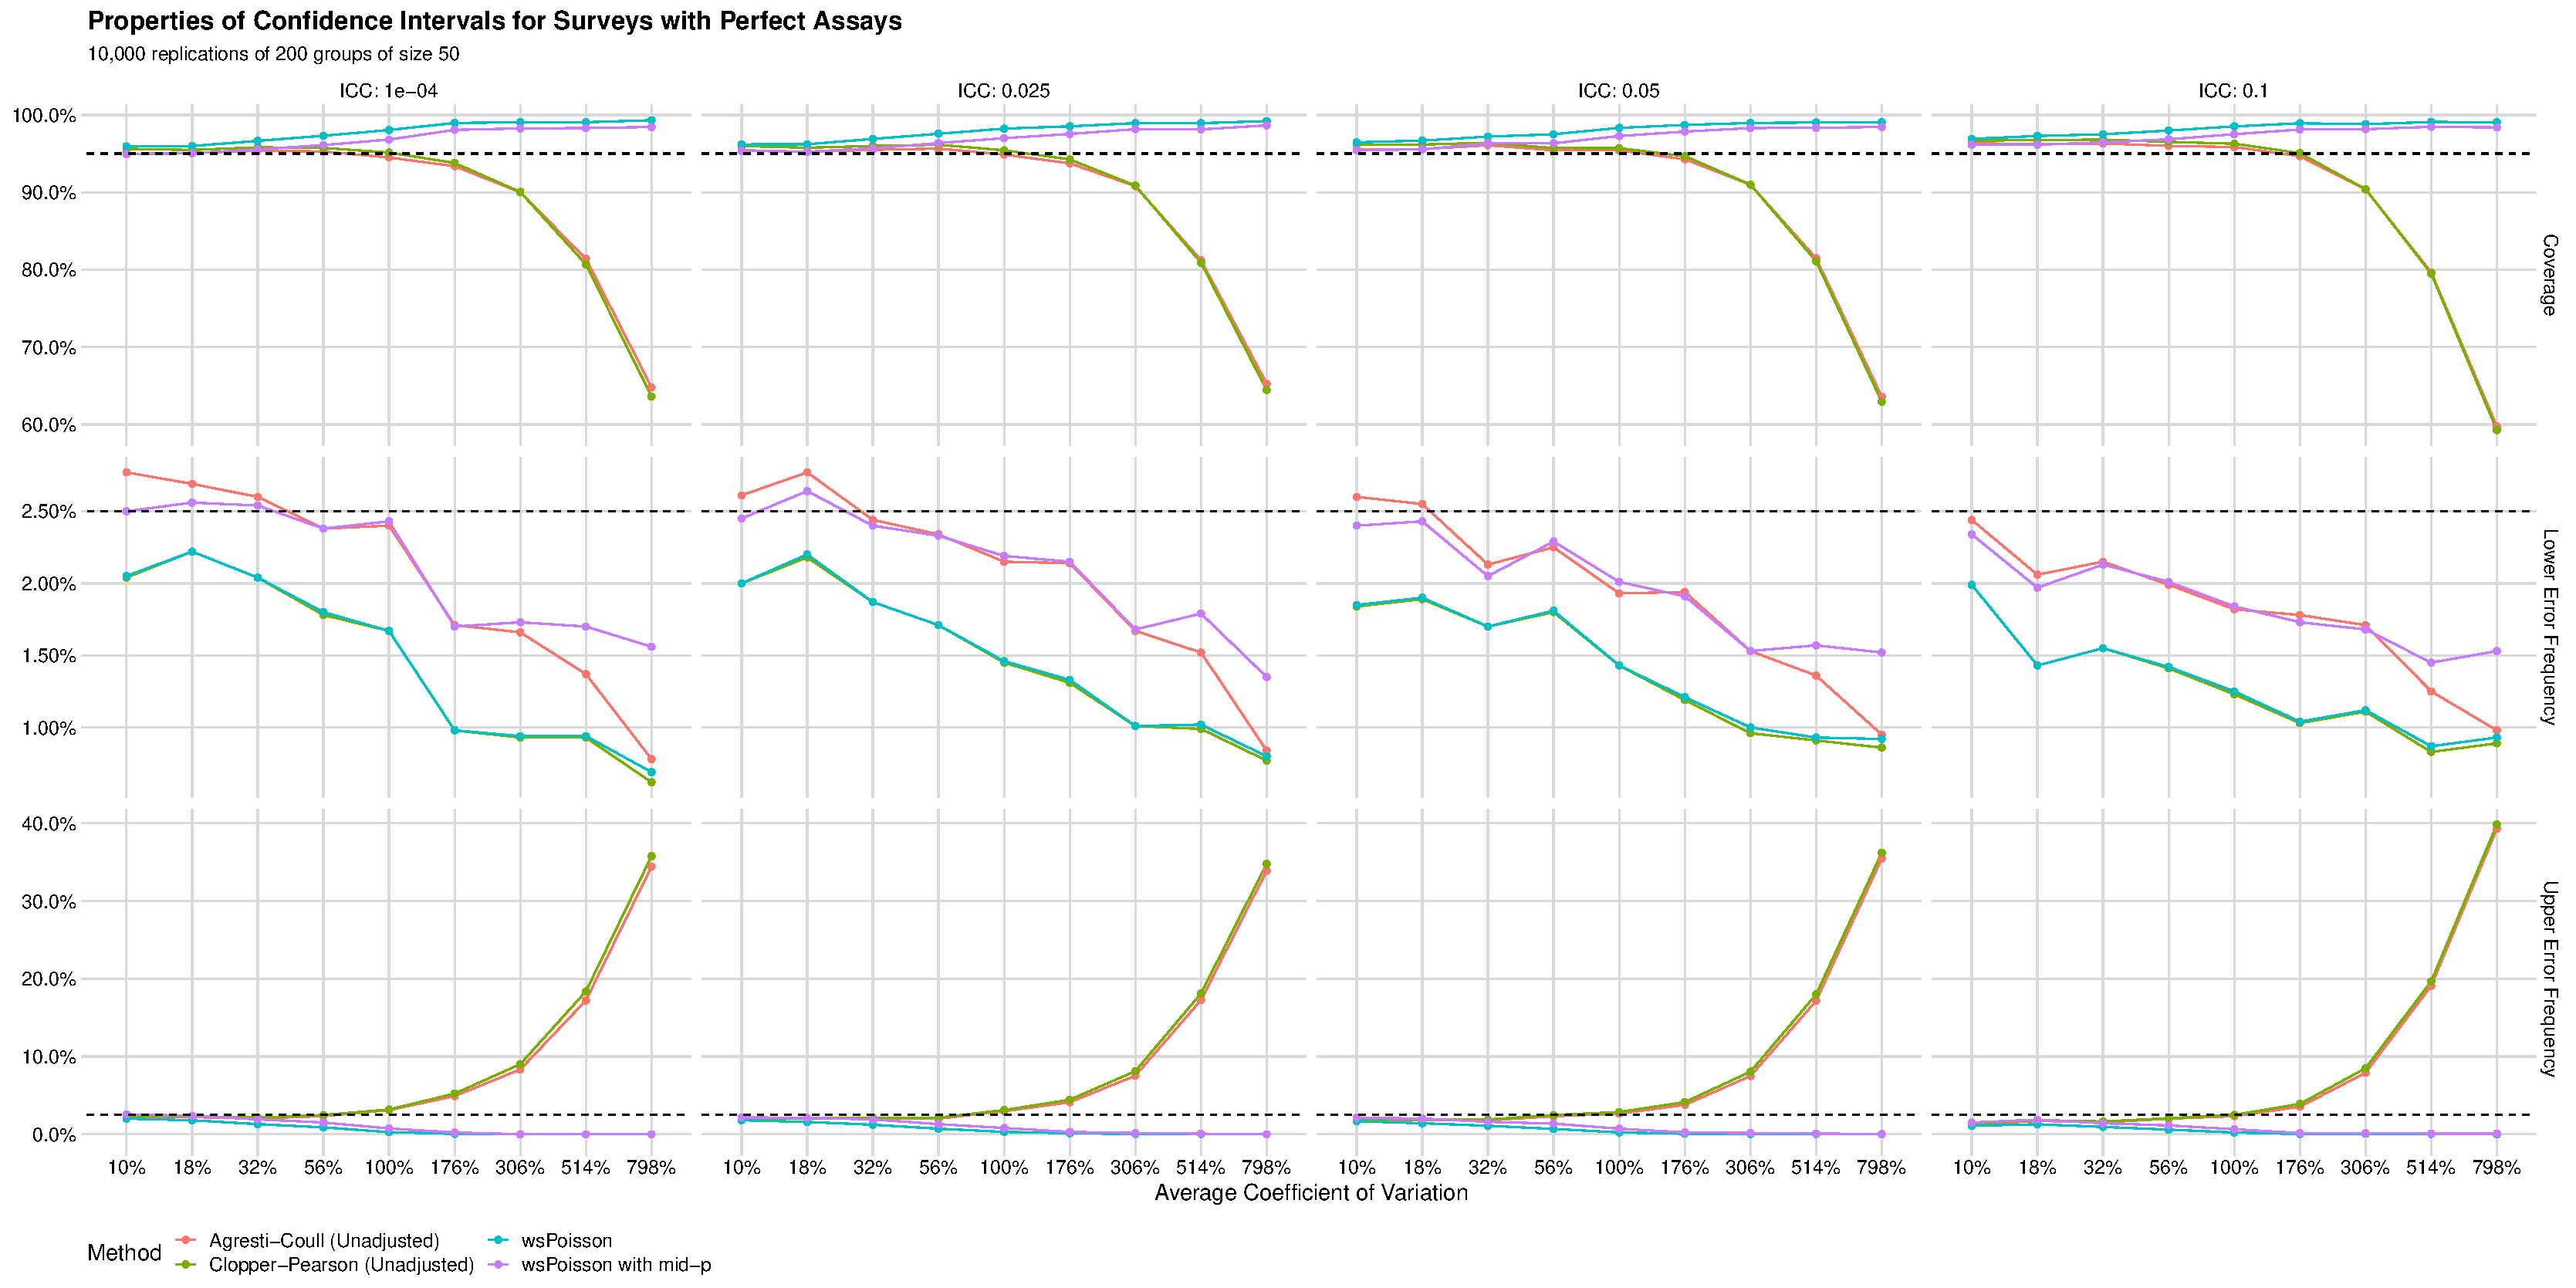
\includegraphics[width = \paperwidth]{figures/results_plot_200_50.pdf}
    \caption{Dirichlet Weights Scenario 2}
    \label{fig:dws2}
\end{figure}
\end{landscape}
\pagebreak







As you predicted, the usual methods (Agresti-Coull and Clopper-Pearson) exhibit poor performance when there is high variance among the weights.

Dean and Pagano recommend an adjustment suggested by Korn and Graubard that I wasn’t sure how to apply in the context of my simulation, so it’s possible that this is a pessimistic assessment of those methods. 

Let’s chat about these results and next steps early next week.

Thanks,

Damon



\subsection{Weird U.S. State Simulation Results}

For this section I have applied 4 methods to 2 populations, with 10,0000 replications each.

\noindent Methods:
\begin{itemize}
    \item AC \& AC\_adj: The Agresti-Coull and Agresti-Coull adjusted methods for survey samples described in \cite{Dean:2015}. Implemented by hand.
    \item wspoissonTest \& wspoissonTest\_midp: the methods described in \cite{FayF:1997} and \cite{FayK:2017}. Implemented in \cite{asht}.
\end{itemize}

In each scenario, I use the 2020 census population counts for all states \& DC and specify the exact number of cases in each state's population to achieve an overall prevalence $\approx$  0.5\%.
Per \cite{Lemeshow1985SurveysTM}, I implement a 2-stage sampling algorithm, where $m$ states are sampled with replacement and $\tilde{n}$ people are sampled from each of the $m$ states.
In the results here, $m = 12,000$ and $\tilde{n} = 1$, equivalent to a simple random sample from the country.
Alternative schemes like $m = 120$ and $\tilde{n} = 100$ seem to produce worse results for the wspoissonTest methods, but I have not investigated this fully.\\
The differences between the two scenarios are presented below.\\

\noindent Scenarios:
\begin{itemize}
    \item one\_state: Montana has 30\% prevalence, while all other states have no cases.
    \item two\_state: California and New York each have 3\% prevalence, while all other states have no cases.
    \item few\_state: California, Texas, Florida, and New York each have 1.5\% prevalence, while all other states have no cases.
    \item many\_state: all states have $\approx$ 0.5\% prevalence, but with some clustering of cases
\end{itemize}

\noindent Results:
\begin{table}
\centering
\begin{tabular}{llrrr}
\toprule
scenario & method & coverage & lower\_error\_freq & upper\_error\_freq\\
\midrule
one\_state & AC & 0.9660 & 0.0232 & 0.0108\\
one\_state & AC\_adj & 0.9660 & 0.0232 & 0.0108\\
one\_state & wspoissonTest & 0.9928 & 0.0039 & 0.0033\\
one\_state & wspoissonTest\_midp & 0.9852 & 0.0083 & 0.0065\\
\addlinespace
two\_state & AC & 0.9484 & 0.0256 & 0.0260\\
two\_state & AC\_adj & 0.9484 & 0.0256 & 0.0260\\
two\_state & wspoissonTest & 0.9632 & 0.0193 & 0.0175\\
two\_state & wspoissonTest\_midp & 0.9538 & 0.0235 & 0.0227\\
\addlinespace
few\_state & AC & 0.9570 & 0.0259 & 0.0171\\
few\_state & AC\_adj & 0.9570 & 0.0259 & 0.0171\\
few\_state & wspoissonTest & 0.9629 & 0.0216 & 0.0155\\
few\_state & wspoissonTest\_midp & 0.9559 & 0.0250 & 0.0191\\
\addlinespace
many\_state & AC & 0.9515 & 0.0287 & 0.0198\\
many\_state & AC\_adj & 0.9515 & 0.0287 & 0.0198\\
many\_state & wspoissonTest & 0.9597 & 0.0246 & 0.0157\\
many\_state & wspoissonTest\_midp & 0.9517 & 0.0281 & 0.0202\\
\bottomrule
\end{tabular}
\end{table}

I have not found any scenarios that ``break" the AC methods, which appear to be on par with the wspoissonTest\_midp methods.
There is no obvious pattern in coverage vs number of states with cases, other than that the wspoissonTest appears to do better with more evenly spread cases and both wspoissonTest methods do poorly in the one\_state scenario.

\section{Confidence Interval on $\beta$ with an Imperfect Assay}
\label{sec-betaImperfect}


\subsection{Preliminaries}

This is the final problem (described in Section~\ref{sec-math} that combines the two other problems.

We have
\begin{eqnarray*}
\beta & = & \sum_{i=1}^{k} w_i \theta_i^*  \\
& = &  \sum_{i=1}^{k} w_i  \frac{ \theta_i - \phi_n }{ \phi_p - \phi_n} \\
& = &   \frac{ \sum_{i=1}^{k} w_i  \theta_i  }{ \phi_p - \phi_n} - \frac{ \phi_n \sum_{i=1}^{k} w_i    }{ \phi_p - \phi_n} \\
& = &   \frac{ \sum_{i=1}^{k} w_i  \theta_i  }{ \phi_p - \phi_n} - \frac{ \phi_n     }{ \phi_p - \phi_n},
\end{eqnarray*}
where the last step is because the weights are assumed to sum to 1.

We can use
\begin{eqnarray*}
\hat{\beta} & = &   \frac{ \sum_{i=1}^{k} w_i  \hat{\theta}_i  }{ \hat{\phi}_p - \hat{\phi}_n} - \frac{ \hat{\phi}_n   }{ \hat{\phi}_p - \hat{\phi}_n} 
\end{eqnarray*}
as our estimator of $\beta$. 

\subsection{Confidence Distribution Approach}

Then we can use the melding method of \citet{FayP:2015} to combine the confidence distributions for $\beta_a = \sum_{i=1}^{k} w_i  {\theta}_i$, for $\phi_p$,
and for $\phi_n$. That might not be straightforward, since I am not sure if $\phi_n$ and $\phi_p$ are monotonic in $\beta$. You need to check that out.

\subsection{Korn-Graubard+CD Approach} 

This is the method described in the supplement of \citet{Kali:2021}.
Basically, we use the method of Korn and Graubard to get confidence distributions for ${\beta}_a = \sum_{i=1}^{k} w_i \theta_i$ (the apparent prevalence, assuming perfect sensitivity and specificity).
Let $\hat{\beta}_a= \sum_{i=1}^{k} w_i X_i$. Under the Poisson assumption, we estimate the variance 
of $\hat{\beta}_a$ with $\widehat{Var}(\hat{\beta}_a) = \sum_{i=1}^{k} w_i^2 X_i$. Then Korn-Graubard define the effective sample size by setting the $\widehat{Var}(\hat{\beta}_a)$ to the binomial variance estimate,
\begin{eqnarray*}
\widehat{Var}(\hat{\beta}_a) \stackrel{set}{=} \frac{\hat{\beta}_a (1-\hat{\beta}_a)}{n_e}
\end{eqnarray*}
So we get 
\begin{eqnarray*}
n_e =   \frac{\hat{\beta}_a (1-\hat{\beta}_a)}{\widehat{Var}(\hat{\beta}_a)}
\end{eqnarray*}
Then the effective count is $x_e = n_e \hat{\beta}_a$, and the lower and upper confidence distributions for ${\beta}_a$ under the Korn-Graubard method are Beta$(x_e, n_e-x_e+1)$ and Beta$(x_e+1,n_e-x_e)$, respectively. 
Then those confidence distributions are used in place of the confidence distributions for $\beta_a$ in the previous subsection. 



%\bibliographystyle{agsm}
\bibliographystyle{biom}


\bibliography{refs}

\end{document} 